\chapter{Application (practical)}
This part will discuss our model's practical implementation alternatives and programming tools. The work will explore three alternatives for implementing text-to-model transformation. \cite{t2m_1} used \textit{Java} as the programming tool in their work, yet their work was published 12 years ago, and during this period, a lot of tools in Artificial intelligence emerged. Therefore, the first step is to reconstruct and implement the current state-of-art approach with more up-to-date technologies. The practical implementation should also be divided into three parts: pre-processing, processing, and post-processing, which correspond to the theoretical design in the last chapter.


\begin{figure}[h]
    \centering
    \caption{Logical partition of approach's functions}
    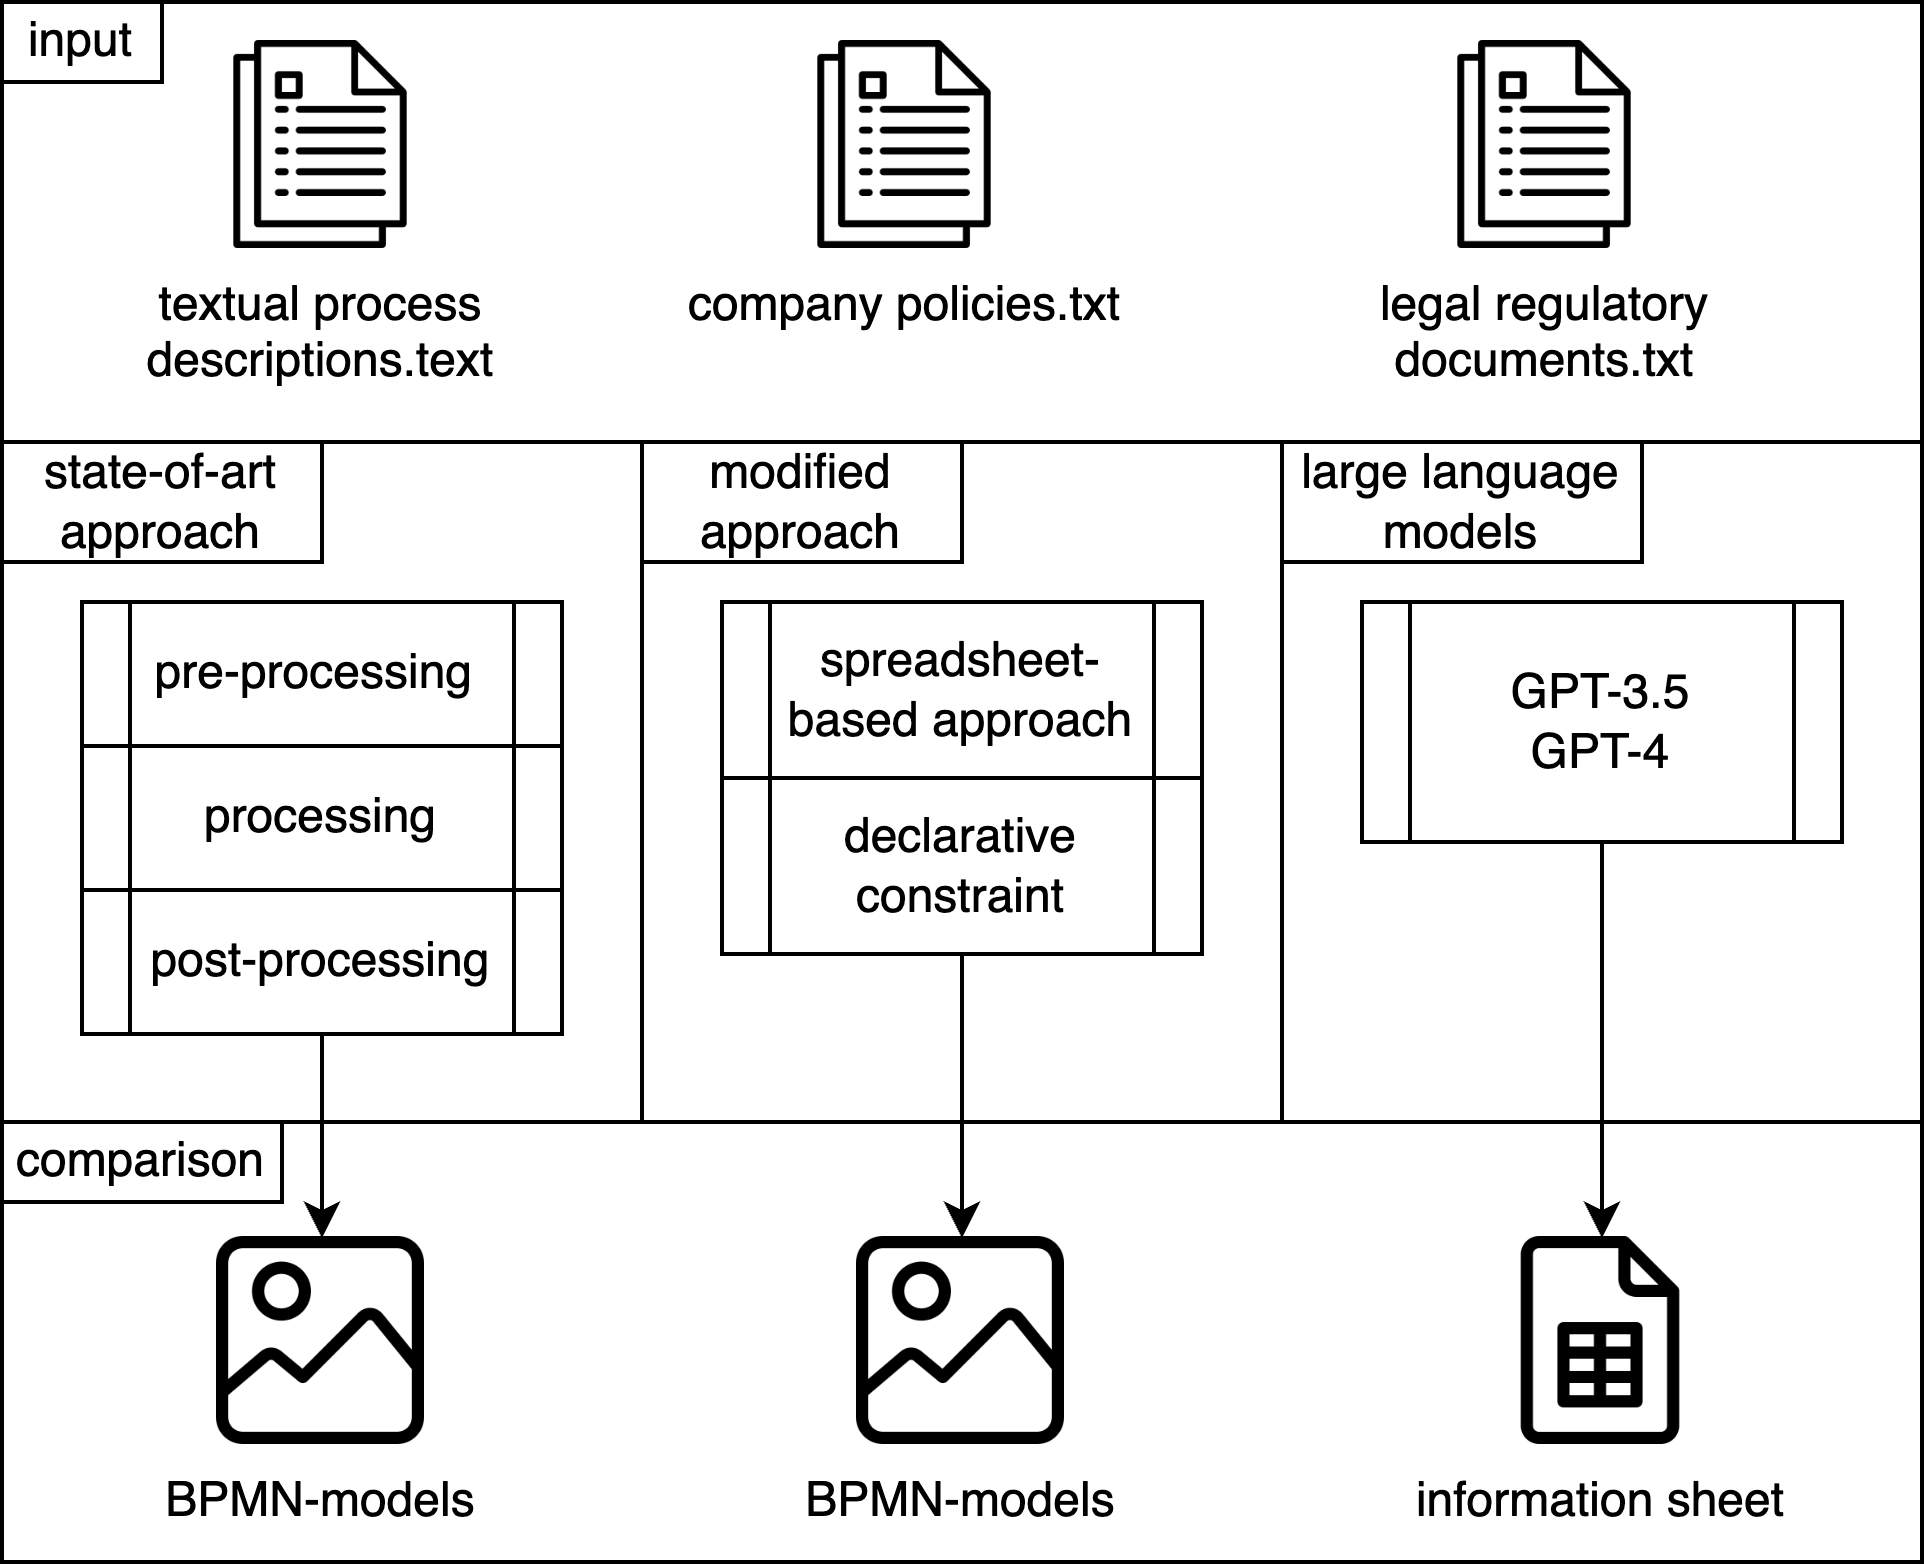
\includegraphics[width=0.9\textwidth]{tum-resources/images/3-approaches.png}
    \floatfoot{Overview of the practical implementation of the proposed approach}
\end{figure}


After thorough research, \textit{Python} as the programming language with the \textit{Spacy}\footnote{https://spacy.io} is decided. \textit{Spacy} is an open-source library for performing natural language processing tasks. This library is chosen because it has a good accuracy of 90.53\% on average with a relatively good execution time \cite{complement_1}. The approach will initially take the textual process descriptions with the format of .txt as input. 


According to the theoretical design, the input file should be broken into words and tagged with correct grammatical labels. \textit{Spacy} integrates these functions in its core and will make the document pre-processing efficient. The processed sentences are stored in a python \textit{doc} class, which is an object that stores a series of natural language properties of the words, e.g. tokenization, part-of-speech tagging, entity recognitions \cite{complement_1}. Several works, \cite{t2m_1} \cite{t2m_2} \cite{t2m_4}, also suggest that the \textit{Stanford parser} is a widely adopted part-of-speech tagging tool with good recognition accuracy and a wide range of \textit{Stanford Dependencies}, which represents the grammatical relationships between words. The work will try to compare these two part-of-speech tagging tools. 

The information stored in the python \textit{doc} class will be used for the main procedure of text-level analysis. \cite{literature_review_4} \cite{t2m_1} address the anaphora resolution problem using the \textit{WordNet} and \textit{FrameNet}, which are a lexical database of English used to perform semantic analysis. To detect conditional markers, a list of signal words can be predefined. while \cite{t2m_1} gives four indicators to identify the signal words: ConditionIndicators, ParallelIndicators, ExceptionIndicators, and SequenceIndicators, which accordingly represents the exclusive gateway, parallel gateway, error intermediate events and continuation of a branch of a gateway. \cite{t2m_1} also gives a good illustration of how to generate the flows between activities, which represent their interactions. 


Finally, the identified business activities connected using flows can be used to generate BPMN models. A list of rules can be created to convert the flows into the process models. In this step, the work will use the flow information to establish connections between business activities. The start and end activities will first be determined by looking into the semantic meanings of the business activities. End activities should be recognized because once an action leads to an end activity, the node should no longer be connected to other nodes. Then, the work will use the conditional relationship to create the corresponding conditional flows. Then, all the business activities can be joined together. Once such connections are established, they will be converted into images.\cite{literature_review_1} also suggests a list of BPMN modeling tools that can be leveraged to generate process models, which this work will look further into. 

After these processes, A prototype replicating the current state-of-art approach in business model auto-generation is available, but implemented using \textit{Python} and \textit{Spacy}, which is more up-to-date and offers better performance. In the second step, relevant works will be analyzed, and constructive thoughts and ideas will be leveraged to improve the developed prototype qualitatively and quantitatively. The qualitative improvement, on the one hand, aims to extend the functions and usability of the prototype. \cite{t2m_6} suggests a spreadsheet-based process model extraction where a spreadsheet is generated and serves as an intermediate media between textual process description and business process model. The spreadsheet provides a good overview of the entire process and allows the human user to check the correctness of the generated process models. Quantitative improvement, on the other hand, refers to the improvement whose aim is to increase the accuracy of the proposed approach.\cite{t2m_5}, and its subsequential work \cite{complement_1}, develop the idea of using rule-based matchers to identify the business process element and summarize a list of XOR and AND gateways to identify the conditional relationships between sentences. \cite{t2m_2} focuses on further exploring the relationship between words and designs an algorithm to generate the declarative constraint, allowing the approach to deal with more kinds of input text form.

In the second step, the prototype's performance with input text of different complexity levels will also be examined. The general textual process description will be used as input to generate process model. Yet, this work intends to find out the range of the usability of the developed prototype. Therefore, company policies and legal regulatory documents will then be used which are different structured compared to general textual process description to determine the adaptability of the prototype.


Finally, in the last step, this work will compare the performance of the developed prototype with the large language models, like \textit{GPT-3.5} or \textit{GPT-4} \footnote{https://platform.openai.com/docs/models}. \textit{GPT-3.5} models are described as being able to understand and generate natural language, while OpenAI describes the \textit{GPT-4} as a large multimodal model and is able to solve complex problems with greater accuracy. Currently, \textit{GPT} models can yet generate process models in the form of images, but we will prompt it to generate a spread containing all process model related information. By comparing these with our prototype, this work is able to gain a deeper understanding of the strengths and limitations of our work and gain insight into future works.

